\documentclass[conference]{IEEEtran}
%\documentclass{article}
\usepackage[utf8]{inputenc}
\usepackage{amsmath}
\usepackage{amssymb}
\usepackage[numbers]{natbib}
\usepackage{graphicx}
\usepackage{color}
\usepackage{soul}


\title{Holographic Emulation by using Fish Tank Virtual Reality, Stereographic Display and Virtual Screen}
\sethlcolor{black}
\author{
\IEEEauthorblockN{\hl{Leonardo Marques Rocha}}
\IEEEauthorblockN{\hl{Homer Simpson}}
\IEEEauthorblockA{\hl{Twentieth Century Fox}\\
\hl{Springfield, USA}\\
\hl{Email: homer@thesimpsons.com}}
\and
\IEEEauthorblockN{\hl{Marcelo da Silva Hounsell}}
\IEEEauthorblockA{\hl{Starfleet Academy}\\
\hl{San Francisco, California 96678-2391}\\
\hl{Telephone: (800) 555--1212}\\
\hl{Fax: (888) 555--1212}\\
\hl{Email: margie@thesimpsons.com}}
\and
\IEEEauthorblockN{\hl{Andre Tavares da Silva}}
\IEEEauthorblockA{\hl{Starfleet Academy}\\
\hl{San Francisco, California 96678-2391}\\
\hl{Telephone: (800) 555--1212}\\
\hl{Fax: (888) 555--1212}\\
\hl{Email: bart@thesimpsons.com}}
}
\begin{document}

\maketitle

\begin{abstract}
This work proposes a new visualization technique to emulate an holographic display with off-the-shelf hardware. Holographic visualization demands an insurmountable volume of data to process and specialized hardware. The stereo visualization technology is common place now and can be combined with existing visualization techniques in order to emulate a hologram. Stereo visualization is combined with Head Coupled Perspective (HCP) in a Fish Tank Virtual Reality (FTVR) environment. These combined techniques create a virtual screen where the hologram is projected with the depth cues for natural immersion in Virtual Reality. Another contribution of this paper is an accompanying visualization pipeline, that delivers consistent and comprehensive 3D graphics in a standard framework.
\end{abstract}

\section{Introduction}
\label{sec.introduction}

This work proposes a new stereo visualization technique to generate the immersion of an holographic display without specialized hardware. Holographic displays are not consolidated because they need special hardware and high computational power~\cite{Lucente1992, Watlington1995, Lucente2012}; but it has the benefit of reproducing the light in all directions, from all viewpoints. The stereo visualization technique already present in the stereo monitors, TVs and movie screens have a limited immersion and a fixed viewpoint. If the content is computer generated, the tracking of the viewer can reproduce the viewpoint, but has limitations on the number of simultaneous viewers~\cite{Harris2010}.

Another contribution of this paper is an holographic transform using the existing OpenGL pipeline. Closely tied in to viewing parameters is 3D interaction, OpenGL standard has emerged to supply the lack of standardization, the need of higher development and support efforts; as well as stifling the proliferation of user interface features like stereo. A standard viewing software toolkit, along with a standard motion toolkit, would benefit end users by delivering consistent and comprehensive 3D interaction across applications.

The section is organized as follows: Section~\ref{sec.holography} provides and introduction in hologram generation; then Stereo is briefly discussed in Section~\ref{sec.stereographic_displays}; and followed by Section~\ref{sec.projection_review}, that reviews the OpenGL 3D projection. The following Sections~\ref{sec.hologram_emulation} and~\ref{sec.holographic_projection} propose an alternative to computer generated hologram and a new projection transform for hologram emulation, respectively, using stereo view pairs.



\section{Fundamentals of Stereo Vision}
\label{sec.stereo}

There are two primary factors to generate a 3D stereo vision, convergence and binocular parallax~\cite{okoshi2012}. The convergence is the angle formed by the eyes and the observed object. The higher the angle value is, the nearer the object is perceived, and vice versa. Therefore, when the convergence is fixed, any object between the eyes and the convergence point will be closer, while the object beyond the convergence point will be farther away. If the convergence is higher then $6^{\circ}$, the eyes feel uneasy~\cite{Fernando2004}. On the contrary, when the value is too small, the stereo sensation will be lost.

Binocular parallax is the difference of images seen by each eye when viewing a scene, creating a sense of depth~\cite{li2012}. The	parallax images are the images passing through to left and right eyes. All 3D stereo media contain a pair of parallax images that are projected on the display, as in Figure~\ref{fig.stereo_parallaxes}. If the images in the pair superimpose, then the binocular focus is on the plane of the images and there is zero parallax.

The positive parallax happens when the target object offsets to the left in the left image, and offsets to the right in the right image, then the binocular focus is lead to fall behind the display, shown in Figure~\ref{fig.stereo_parallaxes}. On the opposite case, the binocular focus is in front of the display, the target offsets are reversed, causing a negative parallax illustrated in Figure~\ref{fig.stereo_parallaxes}.

\begin{figure}
\centering
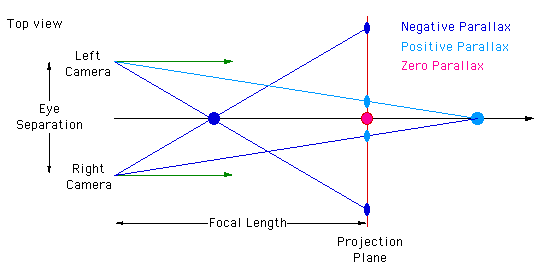
\includegraphics[width=0.8\linewidth,keepaspectratio=true]{figs/stereo_parallaxes.png}

%\begin{tabular}{ccc}
%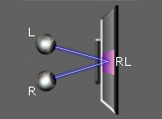
\includegraphics[width=0.3\linewidth,keepaspectratio=true]{figs/zero_parallax.png}
%&
%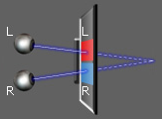
\includegraphics[width=0.3\linewidth,keepaspectratio=true]{figs/positive_parallax.png}
%&
%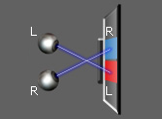
\includegraphics[width=0.3\linewidth,keepaspectratio=true]{figs/negative_parallax.png}
%\\
%(a)&(b)&(c)\\
%\end{tabular}
\caption{Zero, positive and negative stereo parallaxes. }
\label{fig.stereo_parallaxes}
\end{figure}

\subsection{Stereo Displays}
\label{sec.stereo_displays}

The technology for the projection of stereo imagery needs to display (at least) two separate images for left and right eye, respectively, with adequate separation in order to avoid crosstalk or “ghosting”~\cite{Fernando2004}. In general, all existing stereo technology displays the simultaneous projection of two images, so that only one stereo view point can be displayed. 

%In auto-stereographic displays, the emitted viewing rays are blocked or not by a parallax barrier in front of the display, or diverted by a lenticular screen~\cite{Konrad2007}. Although that, only two view points are necessary to create the stereo image pair. A lot of auto-stereographic technologies have been proposed but only few are ready for the end user~\cite{Harris2010}. 

In modern stereo displays, each stereo view point is combined in several ways on the screen; with intertwined lines or squares, combined in even-odd line positions or chessboard pattern respectively; with split screen, divided horizontally or vertically, where each view point is assigned to the respective split side; and with temporal modulation, that requires synchronization with the view polarization apparatus, in the common case stereo glasses with active shutters. Glasses without synchronization relies on passive polarization, that works for all but latter stereo view combination and doubles the resolution per inch halving the amount of pixels.

Active stereo with shutters is based on the principle that the left and right eye images are projected sequentially by a single projector, and that the viewers wear shutter glasses to selectively view the left and right eye images. In order to achieve a good, flicker-free image, the refresh rate needs to be at least 96 Hz (which yields 48 Hz per eye)~\cite{Fernando2004}. The good aspect is, only one display is required for the projection of both left and right images and the effect is independent on the screen type that is used. The drawback are the glasses, which are heavy, cumbersome and needs constant line-of-sight connection with the infrared emitter. Some users also report headaches after extended use.

Passive stereo based on light polarization is a very straightforward technology, using the fact that polarized lenses block the perpendicular light whereas parallel light is transmitted. In its most simple implementation, polarized lenses are mounted in any type of projector. 

%Recent development~\cite{Fernando2004}, using spectral filters to separate between the left and right eye images. This combines the benefits of active and passive: a regular screen can be used, the glasses are lightweight and passive, and the separation is excellent in a restricted angle of viewing.

\section{3D Visualization Pipeline}
\label{sec.visualization_pipeline}

%This section reviews the viewing transform used by most popular graphics frameworks such as OpenGL. 

%Yet there is no standard way to specify the view, and there are a wide range of different viewing implementations currently in use.

%Closely tied in to viewing parameters is 3D interaction, and there are likewise a large number of different 3D interaction implementations often providing the same basic functionality. Users are forced to learn and use different pan, zoom, and spin techniques for each 3D program they use. As every 3D program has to reinvent this functionality,  OpenGL standard has emerged to supply the lack of standardization, the need of higher development and support efforts; as well as stifling the proliferation of user interface features like stereo. A standard viewing software toolkit, along with a standard motion toolkit, would benefit end users by delivering consistent and comprehensive 3D interaction across applications, and would benefit developers by reducing development time, software support, and customer support. All of the various interaction techniques can be provided to satisfy the varying requirements of the different types of 3D programs and the different levels of end user expertise.

The generation of 3D computer graphics is essentially a straightforward mapping of graphical items in a 3D volume, in a spatial domain $S$ in $\Re^3$, to a 2D image, in a spatial domain $S^{\prime}$ in $\Re^2$. Most viewing software use different transforms combined to deliver consistent and comprehensive 3D interactions: the model transform represents affine transformations, scale, translation and rotation, of each object in the 3D scene in the mapping $M_{model}: S_{model} \Rightarrow S_{scene}$; the view transform represents the individual transformations of every object in the 3D scene, representing the scene positioning for the viewer; which is the mapping $M_{view}: S_{view} \Rightarrow S_{scene}$; and the projection transform is the mapping $M_{proj}:S_{view} \Rightarrow S_{proj}$ that represents the perception of depth of the eye or camera. The final transform to 2D screen coordinates is $M_{screen}:S_{proj} \Rightarrow S^{\prime}_{screen}$. Note that in $M_{model}$ and $M_{view}$ the mapping is inverted to preserve the original spatial domain. Without loose of generality, all mappings can be defined as matrix transforms.

%The combination of the first and second transforms, view and model, is a single transform that translates and rotates the scene accordingly the viewer position, looking direction and view roll. This is an affine transform and the inverse  transform exists. Both transforms can be easily computed as a matrix in homogeneous coordinates. The latter transform projects the 3D scene into the output image. In most cases, the output image is a rectangular shape and the 3D view volume, called frustum, which is either a rectangular prism or a truncated pyramid for parallel and perspective views, respectively.


\subsection{OpenGL Pipeline}
\label{sec.opengl_pipeline}

In the OpenGL framework, the model and view transforms are combined in the \verb|GL_MODELVIEW| matrix. The 3D scene rendered by OpenGL must then be projected onto the computer screen using the \verb|GL_PROJECTION| matrix. In perspective projection, transforms a 3D point in a pyramid frustum in eye coordinates, truncated at the top, by the near plane $n$, and in the bottom, by the far plane $f$. The pyramid is bounded in $n$: in the horizontal by left and right coordinates, $l$ and $r$, and in the vertical by bottom and top coordinates, $b$ and $t$, respectively. The frustum is normalized in Normalized Device Coordinates (NDC), that is a mapping into a cube with the range of $x$-coordinate from $[l, r]$ to $[-1, 1]$, the y-coordinate from $[b, t]$ to $[-1, 1]$ and the $z$-coordinate from $[n, f]$ to $[-1, 1]$. The eye coordinates are defined in the left-handed coordinate system, but NDC uses the right-handed coordinate system. That is, the camera at the origin is looking along $-Z$ axis in eye space, but it is looking along $+Z$ axis in NDC. Since the OpenGL command glFrustum() accepts only positive values of near and far distances, they are negated during the construction of \verb|GL_PROJECTION| matrix.

\begin{figure}[h!]
\centering
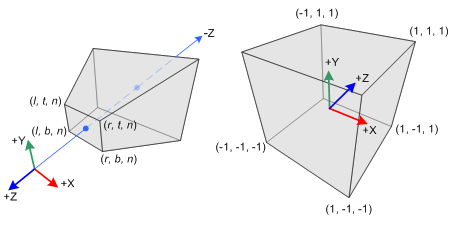
\includegraphics[width=0.9\linewidth,keepaspectratio=true]{figs/gl_projectionmatrix01.png}
\caption{Perspective Frustum and Normalized Device Coordinates (NDC)}
\label{fig.ndc}
\end{figure}

Part of the scene that is not going to be displayed, i.e., all vertex outside the frustum, is removed by frustum culling (clipping) and the edges of the polygon where clipping occurs are reconstructed. This is done transforming all vertex data from the eye coordinates, $(x_e, y_e, z_e)$, to the clip coordinate to clip coordinates $(x_c, y_c, z_c)$ in Equation~\ref{eq.clip}: 

\begin{equation}
\begin{aligned}
\begin{pmatrix} x_{c}\\y_{c}\\z_{c}\\w_{c} \end{pmatrix} &= 
M_{proj} \cdot \begin{pmatrix} x_{e}\\y_{e}\\z_{e}\\w_{e} \end{pmatrix}\\
%\begin{pmatrix} x_{ndc}\\y_{ndc}\\z_{ndc}\end{pmatrix} &=
%\begin{pmatrix} x_{c}/w_{c}\\y_{c}/w_{c}\\z_{c}/w_{c} \end{pmatrix}\\
\end{aligned}
\label{eq.clip}
\end{equation}

The clipping is performed in the clip coordinates by comparing with $w_c = -z_e$. If any clip coordinate is less than $-w_c$, or greater than $w_c$, then the vertex will be discarded. Then, those clip coordinates are also transformed to NDC by dividing the coordinates by the $w_c$ component in Equation~\ref{eq.ndc_coords}.
Bear in mind that both clipping and NDC transformations are integrated into \verb|GL_PROJECTION| matrix.

\begin{equation}
\begin{aligned}
\begin{pmatrix} x_{ndc}\\y_{ndc}\\z_{ndc}\end{pmatrix} &=
\begin{pmatrix} x_{c}/w_{c}\\y_{c}/w_{c}\\z_{c}/w_{c} \end{pmatrix}\\
\end{aligned}
\label{eq.ndc_coords}
\end{equation}

Then, a 3D point in eye space is projected onto the near plane. The following diagrams show how a point $(x_e, y_e, z_e)$ in eye space is projected to $(x_p, y_p, z_p)$ on the near plane.

\begin{figure}[h!]
\centering
\begin{tabular}{cc}
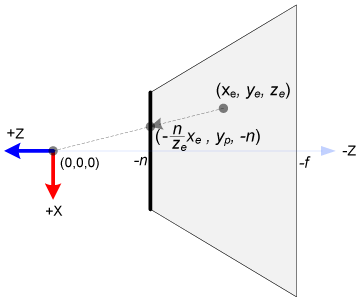
\includegraphics[width=0.45\linewidth,keepaspectratio=true]{figs/gl_projectionmatrix03.png}
&
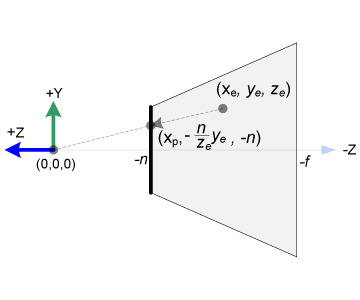
\includegraphics[width=0.45\linewidth,keepaspectratio=true]{figs/gl_projectionmatrix04.png}
\\
(a) Top View of Frustum
&
(b) Side View of Frustum
\end{tabular}
\label{fig.frustum}
\caption{Views of the frustum.}
\end{figure}

%From the top view of the frustum, the $x$-coordinate of eye space, $x_e$ is mapped to $x_p$, which is calculated by using the ratio of similar triangles;

%\begin{equation}
%\begin{aligned}
%\begin{split}
%\frac{x_p}{x_e}&=\frac{-n}{z_e}\\
%x_p&=\frac{-n \cdot x_e}{z_e}\\
%   &=\frac{n \cdot x_e}{-z_e}
%\end{split}
%\end{aligned}
%\label{eq.xp}
%\end{equation}

%From the side view of the frustum, $y_p$ is also calculated in a similar way; 

%\begin{equation}
%\begin{aligned}
%\begin{split}
%\frac{y_p}{y_e}&=\frac{-n}{z_e}\\
%y_p&=\frac{-n \cdot y_e}{z_e}\\
%   &=\frac{n \cdot y_e}{-z_e}
%\end{split}
%\end{aligned}
%\label{eq.yp}
%\end{equation}

Note that both $x_p$ and $y_p$ depend on $z_e$; they are inversely proportional to $-z_e$. In other words, they are both divided by $-z_e$. It is a very first clue to construct \verb|GL_PROJECTION| matrix. Therefore, the $w$-component of the clip coordinates is set as $-z_e$. And, the 4th row of \verb|GL_PROJECTION| matrix becomes $(0, 0, -1, 0)$: 

\begin{equation}
\begin{aligned}
\begin{split}
\begin{pmatrix} x_{c}\\y_{c}\\z_{c}\\w_{c} \end{pmatrix} &= 
\begin{pmatrix} 
\cdot & \cdot & \cdot & \cdot \\
\cdot & \cdot & \cdot & \cdot \\
\cdot & \cdot & \cdot & \cdot \\
0 & 0 & -1 & 0 \\
\end{pmatrix} &=
\begin{pmatrix} x_{e}\\y_{e}\\z_{e}\\w_{e} \end{pmatrix}
\end{split}
\end{aligned}
\label{eq.rows}
\end{equation}

%\begin{figure}[h!]
%\centering
%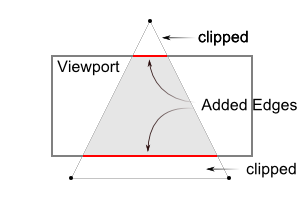
\includegraphics[width=0.9\linewidth,keepaspectratio=true]{figs/gl_frustumclip.png}
%\caption{A triangle clipped by frustum}
%\label{fig.clipping}
%\end{figure}

When all other entries in Equation~\ref{eq.rows} are obtained~\cite{schreiner2004}, the complete projection matrix is: 

\begin{equation}
\begin{aligned}
M_{proj} &= 
\begin{pmatrix} 
\frac{2n}{r-l} & 0 & \frac{r+l}{r-l} & 0 \\
0 & \frac{2n}{t-b} & \frac{t+b}{t-b} & 0 \\
0 & 0 & -\frac{f+n}{f-n} & -\frac{2fn}{f-n} \\
0 & 0 & -1 & 0 \\
\end{pmatrix} \\
\end{aligned}
\label{eq.projection_matrix}
\end{equation}




\subsection{Stereo Visualization}
\label{sec.stereo_visualization}

Let the distance of the eye to the screen, $d_{s}$, and the intra-ocular separation, $d_{io}$. Stereo view is enabled by translating the view off-center to the left by $d_{eye} = -d_{io}/2$,  and to the right by $d_{eye} = d_{io}/2$, as shown in Figure~\ref{fig.stereo_views}a. The view is split for left and right eyes using $M_{eye}$ in Equation~\ref{eq.stereo_view_matrix} combined with $M_{view}$.

\begin{equation}
\begin{aligned}
M_{eye} &= 
\begin{pmatrix} 
1 & 0 & 0 & d_{eye}\\
0 & 1 & 0 & 0\\
0 & 0 & 1 & 0\\
0 & 0 & 0 & 1\\
\end{pmatrix}
\end{aligned}
\label{eq.stereo_view_matrix}
\end{equation}

\begin{figure}[!hb]
\centering
\begin{tabular}{cc}
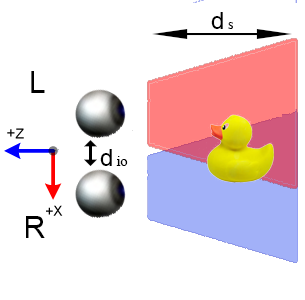
\includegraphics[width=0.35\linewidth,keepaspectratio=true]{figs/stereo_offset.png}
&
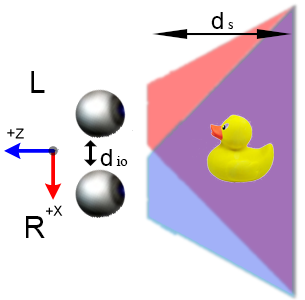
\includegraphics[width=0.35\linewidth,keepaspectratio=true]{figs/stereo_shear.png}
\\
(a)&(b)
\end{tabular}
\caption{Stereo views.}
\label{fig.stereo_views}
\end{figure}

Regarding the stereo technique to display the left and right views, adjustments in the horizontal, $s_x$, or vertical, $s_y$, scales are applied after the stereo view. In case of the modulation of the right and left views along time, there is no split and the view is fully displayed using  $s_x = s_y = 1$. In case of stereo split of the screen, each left and right views are scaled to half by $s_x = 2$, in case of vertical split, or by $s_y = 2$, in case of horizontal split. Both splits can be used to create the intertwined lines of right and left eye polarization.  

The convergence point is moved from $z=-\infty$ towards $+z$ by the shearing, as shown in Figure~\ref{fig.stereo_views}b, of the left and right projection frustum by $sh_z = d_{eye}/d_{s}$. The final stereo projection matrix, $M_{stereo}$, is a matrix scaled by $s_x$ and $s_y$, and sheared $sh_z$ in Equation~\ref{eq.stereo_proj_matrix}. The stereo pipeline is the sequence of transformations: $M_{stereo} \times M_{proj} \times M_{eye} \times M_{view}$.

\begin{equation}
\begin{aligned}
M_{stereo} &= 
\begin{pmatrix} 
s_x & 0 & 0 & 0\\
0 & s_y & 0 & 0\\
0 & 0   & 1 & 0\\
0 & 0   & 0 & 1\\
\end{pmatrix}
\begin{pmatrix} 
1 & 0 & sh_z & 0\\
0 & 1 & 0 & 0\\
0 & 0 & 1 & 0\\
0 & 0 & 0 & 1\\
\end{pmatrix}
\end{aligned}
\label{eq.stereo_proj_matrix}
\end{equation}

 

\section{Holographic Visualization}
\label{sec.holographic_visualization}

Holograms are expected to show visual effects of a 3D scene as a Volume Of Interest (VOI) projected outside the screen. The projection keep all the depth cues of the objects of the VOI: the relative sizes of the objects from the perspective deformation, the stereo depth perception from stereo convergence, binocular parallax and ocular accommodation of the eyes by focusing at different distances; the motion parallax~\cite{li2012} from the difference in the positions of the objects as the viewer moves, the monocular occlusion~\cite{Lucente1995} when one part of image is obstructed by another overlapping part; and pictorial monocular depth cues of texture gradient, aerial perspective, shading, and relative sizes~\cite{Lucente1995}. 

The hologram has an unique feature: viewers are allowed to walk around the VOI and have a \emph{surround viewing}~\cite{debevec2006}, a shared visualization in different angles that is naturally perceived by the eyes without any wearable apparatus. Additionally to that, two or more viewers can view the VOI in different angles because the viewing rays are propagated in a Field of View (FOV) from the holographic apparatus~\cite{Lucente1992}. The current CGH displays have a limited FOV of $60^{\circ}$~\cite{Slinger2005, Lucente1995} due the compromise of the quality of the hologram and computational processing power.

The surround viewing, combined with the depth cues, creates the illusion effect of Pepper's Ghost~\cite{smithwick2014}, which means that the viewer can interact with the VOI with no physical barriers. The practical applications for the combined 3D visualization and interaction can be illustrated, but not limited, in Medical Imaging. For example, a scene of 3D reconstructed organs from 3D medical imagery of 3D Computed Tomography (CT) scans or Magnetic Resonance Imaging (MRI) composes the VOI and is projected as a hologram. The organs are the objects that can be manipulated \emph{in locus} for virtual surgery, and there is no display screen acting as a physical barrier between the object and viewer. Any examination of the organs is provided by the surround viewing and depth cues of the VOI. The surgery simulation is achieved because the spectral illusion is created for the surgeon in a Virtual Reality (VR) environment.

\subsection {Holographic Emulation}
\label{sec.holographic_emulation}

The proposal of this work is to investigate a Virtual Reality (VR) environment that can provide the combined effects of the hologram but that don't have the computational cost of CGH. Most of current VR environments can be composed of off-the-shelf hardware, and the proposed environment does not rely on specialized hardware for CGH to avoid its high costs~\cite{fournier2004}. The proposed VR environment is composed by two 3D standard stereo TVs, combined in a Fish Tank Virtual Reality (FTVR)~\cite{Ware1993} environment and a depth camera. The camera creates a Head Coupled Perspective (HCP)~\cite{okoshi2012}, as shown in Figure~\ref{fig.tv_setup}, by projecting virtual objects considering the location of the viewer, which is acquired by tracking. HCP improves the depth perception~\cite{li2012} and, when combined with stereo vision, can create an holographic emulation. 

The FTVR is combined with HCP and stereo vision to create a virtual screen, which is the perceived screen from the depth cues created by the two stereo displays that are juxtapositioned with a tilt angle of in Figure~\ref{fig.tv_setup}. The surround viewing is achieved by tracking the position of the viewer as in the original FTVR setup. Although HCP is has been reported more important than stereo in 3D visualization~\cite{Ware1993}, the holographic perception is created using the binocular parallax. The HCP viewing is adjusted with negative parallax to create the depth cue of the virtual screen and the spectral illusion of Pepper's Ghost. Other depth cues are adjusted to the viewing angle of the virtual screen using the position tracked by the the depth camera.

\begin{figure}[!hbt]
\centering
%\begin{tabular}{cc}
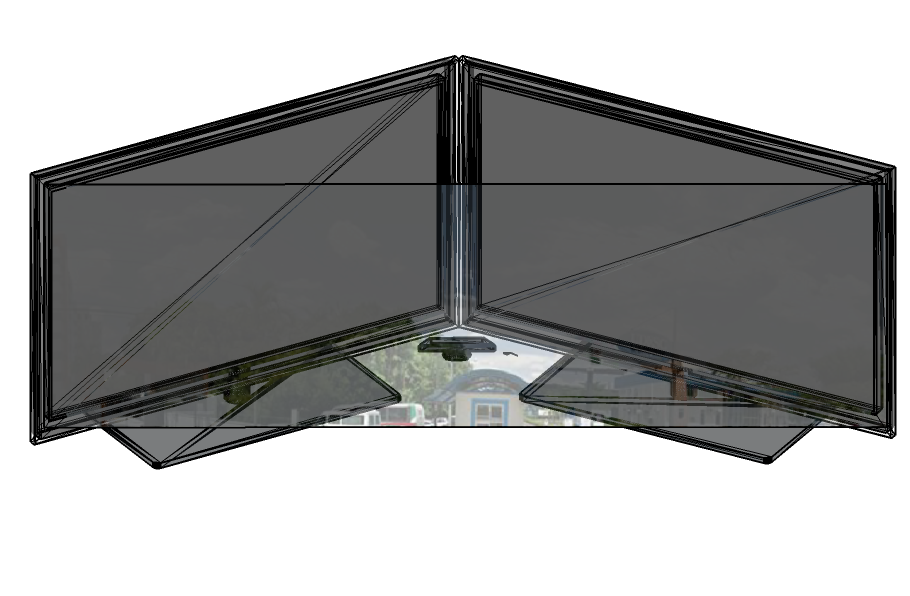
\includegraphics[width=\linewidth,keepaspectratio=true]{figs/labsetup_01.png}
%&
%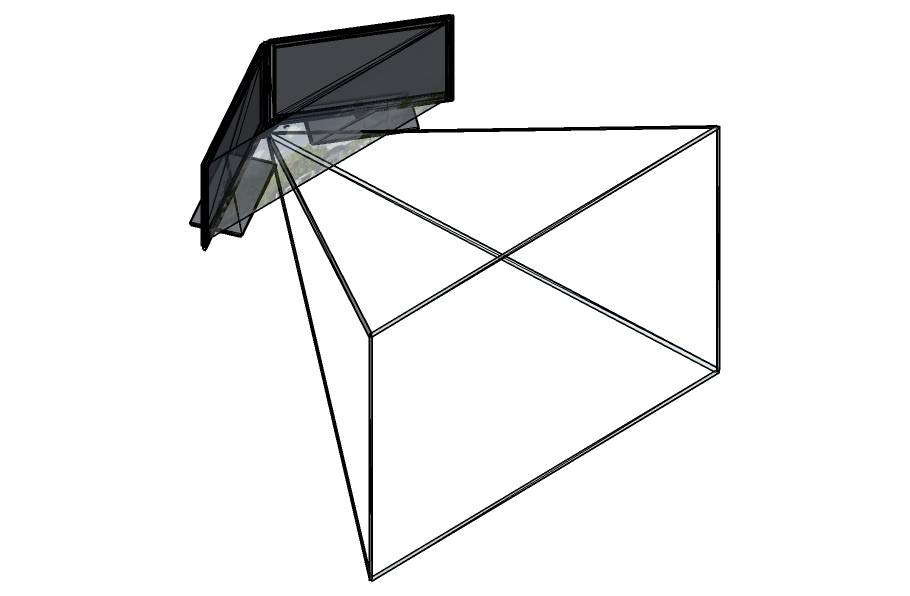
\includegraphics[width=0.4\linewidth,keepaspectratio=true]{figs/labsetup_02.png}\\
%(a) Virtual screen & 
%(b) Tracking frustum
%\end{tabular}
\caption{FTVR setup of the stereo displays and depth camera.}
\label{fig.tv_setup}
\end{figure}

The tracking system has to capture the position of the viewer with high accuracy in order to avoid incorrect HCP. It also needs to be robust to body movement or objects that may partially occlude the viewer. In order to achieve the desired robustness and accuracy, a depth camera is used instead of a standard RGB camera. The depth sensor has a higher accuracy in the estimation of the depth and with this information can remove artifacts in the image that are occluding or degrading the positional information of obtained from the RGB channels. 

Although the proposed emulation has the restriction of a single viewer for simplicity, the proposed setup can be extended up to four viewers. The depth information can be also used to distinguish two people in front of the TVs, and two depth cameras can be combined to track four viewers. The standard stereo TVs with 240 Hz refresh rate can provide stereo pairs up to four viewers with some flickering~\cite{Frohlich2005}. 

%This investigation setups two 3D displays forming the FTVR as in the illustration of Figure~\ref{fig.tv_setup}a. 



%The cornerstone of the proposed projection is how this can be done with the existing viewing pipeline of 3D graphics frameworks such as OpenGL. The existing viewing transformations works well for 3D with positive stereo parallax, showing the object as inside the screen of display. In the opposite case, the projection with negative parallax requires the translation $T_{parallax}$ of the scene towards the virtual display. This is incorporated in the view transformation $M_{view}$ of Section~\ref{sec.projection_review}, creating a translated view $M_{view}T$. Let the modification of the viewpoint produce a new view transform $M^{\prime}_{view}$. This new viewpoint combined with $T_{parallax}$ is then defined as $M^{\prime}_{view} T$. The following projection $M_{projection}$ depends on the value of $z$, which means that the latter translation is not applied not only in the depth, but also in the other directions, moving the scene coordinates with the distance from the screen. 

%In the proposed hologram emulation, the scene should be projected with negative parallax to appear in a distance away from the screen. For the viewer, objects of the scene appears in a fixed position outward from the screen. The immersion depends on the viewer position for eye accommodation, stereo convergence and binocular parallax. Additionally to that, the FOV provided by the FTVR and HCP projection enhances the realism of the scene and the sense of presence~\cite{Hounsell2013}. 

%The HCP projection of the scene provided by the OpenGL pipeline in Section~\ref{sec.projection_review} works for standard stereo projection. In the proposed hologram emulation, the projection has to emulate a virtual Volume Of Interest (VOI) with the stereo negative parallax. The VOI is created with depth cues to emulate the hologram. The perspective cue is dependent on the viewing angle and distance from screen, but not on binocular parallax. 

%There is no motion parallax in the VOI and all objects in the hologram have fixed position.

%The main pipeline of OpenGL follows the sequence of transforms: $M_{model}$, $M_{view}$, $M_{proj}$ and $M_{screen}$. In ordinary HCP, $M_{model}$ setups the scene. $M_{view}$ applies the viewpoint from the tracked position, and $M_{proj}$ sets the depth cues. While the perspective depth cue is set with $M_{proj}$, the binocular parallax is set with the stereo projection of Equation~\ref{eq.stereo_projection_matrix} in Section~\ref{sec.stereo_projection}. This projection has zero parallax for a convergence point in the plane of projection, which is the screen of display, and negative parallax at any convergence point in front of the stereoscopic displays. In order to achieve this, the view transform $M_{view}$ has to create a viewpoint looking towards $-z$, because the horizontal negative parallax has to increase away from the screen with the multiplication of the first term on the right of Equation~\ref{eq.stereo_projection_matrix} and the object coordinates $(x, y, z)$ in the VOI. The result of this multiplication is the coordinate translated in $x$ to create the stereo offset, $(x+ sh_z \cdot z, y, z)$. Therefore, the objects have increasing negative parallax in the increasing positive $z$ axis.

%This projective setup introduces a motion parallax for object that are off-center. This is desired for HCP with positive parallax, but not for the hologram emulation because the VOI does not have motion parallax associated with the viewpoint. If $M_view$ is restricted to invert the orientation of the $z$ axis, and $M_{proj}$ applies the shift in the frustum that aligns that origin with the plane with zero parallax, the far plane in most cases, the motion parallax of the HCP is removed. This also is incorrect  because $M_{view}$ should be applied after the shift to generate the viewpoint for HCP. If applied before, the viewpoint is for a scene that is projected along $-z$ as in glFrustum(). One possible way is to correct to keep $M_{view}$ fixed and adjust the rotation and position of each model $M_{model}$ in order to produce the correct viewing angle, but those are cumbersome operations that are not in the semantics of each transform in the OpenGL pipeline. 

%The Figures~\ref{fig.transformation}a-d show an example of a scene composed of duck 3D model. Figure~\ref{fig.transformation}a shows the scene with the shift its applied before the projection to create negative parallax. If the viewpoint is changed to look the top left corner of the picture, a motion parallax is created, illustrated in Figure~\ref{fig.transformation}b. If the shift is applied after $M_{proj}$, the motion and binocular parallaxes are correct, but not the HCP, and the duck in Figure~\ref{fig.transformation}c is not aligned with the viewpoint in the left top corner.The correct viewing angle, as shown in Figure~\ref{fig.transformation}d, can be adjusted programmatically with $M_{model}$ of each object in the scene.

% remove \iffalse ... \fi block to uncomment
\iffalse

\begin{figure}
\centering
\begin{tabular}{|c|c|}
\hline
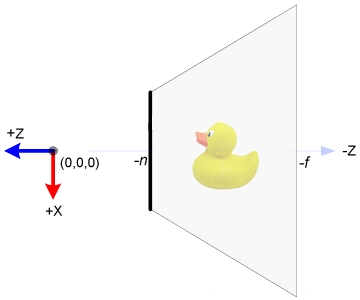
\includegraphics[width=0.45\linewidth,keepaspectratio=true]{figs/scene01.png}
&
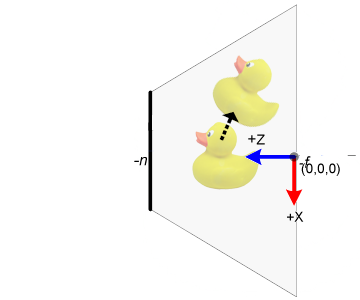
\includegraphics[width=0.45\linewidth,keepaspectratio=true]{figs/scene02.png}
\\
(a)&(b)\\ \hline
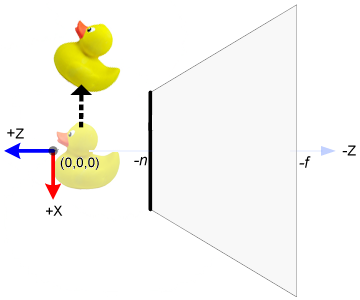
\includegraphics[width=0.45\linewidth,keepaspectratio=true]{figs/scene03.png}
&
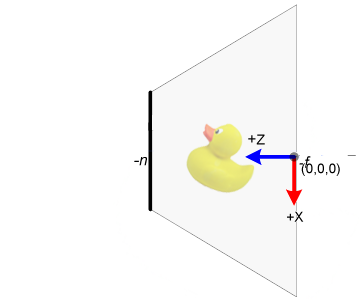
\includegraphics[width=0.45\linewidth,keepaspectratio=true]{figs/scene04.png}
\\ 
(c)&(d)\\ \hline
\end{tabular}
\caption{Example of a scene composed by a duck and the projection frustum of Section~\ref{sec.stereo_projection}. The viewer is at left center in picture (a)  and in the top left corner in pictures (b) to (d).}
\label{fig.transformation}
\end{figure}
\fi







\subsection{Holographic Pipeline}
\label{sec.holographic_pipeline}

The main pipeline presented in Section~\ref{sec.visualization_pipeline} follows the sequence of transforms: $M_{model}$, $M_{view}$, $M_{proj}$ and $M_{screen}$. In ordinary HCP, $M_{model}$ setups the scene. $M_{view}$ applies the viewpoint of the tracked position, and $M_{proj}$ sets the depth cues. The 3D viewing transforms, $M_{view}$ and $M_{proj}$ can be further split into smaller transforms: a \emph{view pipeline} and  a \emph{projection pipeline}, respectively.

In the proposed FTVR, the screens are tilted to create the virtual screen. The transformation matrix for the tilted screen-local coordinates, $M_{tilt}$, maps the Cartesian coordinate system of the virtual screen onto the screen space coordinate system. If a point is lying in the virtual plane, then the transformation $M_{tilt}$ will realign it to lie into the plane of the screen. The screen space basis are the vectors $v_r$, $v_u$, and $v_n$, the vectors for the right, up and normal directions. The mapping of $M_{tilt}$ is the inverse of the holographic mapping into the plane of the virtual screen. In the holographic views, any point lying in the plane of the screen will be realigned to lie in the virtual screen plane. This mapping is produced by the inverse of $M_{tilt}$. Fortunately, $M_{tilt}$ is an orthogonal rotation, and its inverse is its transpose, $M_{tilt}^{T}$, with screen space basis vectors as rows instead of as columns:

\begin{equation}
\begin{aligned}
M_{tilt}^{T} &= 
\begin{pmatrix} 
v_{rx} & v_{ry} & v_{rz} & 0\\
v_{ux} & v_{uy} & v_{uz} & 0\\
v_{nx} & v_{ny} & v_{nz} & 0\\
0      & 0      & 0      & 1\\
\end{pmatrix}
\end{aligned}
\label{eq.tilt_matrix_transpose}
\end{equation}

The viewpoint of the viewer, $M_{cam}$, simulates a camera looking towards $-z$. While the viewpoint can be applied anywhere in the 3D space, the mathematics of perspective projection as defined by matrix $M_{proj}$ disallow this, by the foreshortening division by $z$. The frustum of the camera is forever trapped at the origin, and if we wish to transform the viewpoint, we must instead apply the inverse of this transform to the entire scene. Thus, we instead align the scene with the frustum of the camera. The viewpoint of $M_{cam}$ has to be in tracked position $p_e$, then the scene is translated using the offset of the tracked position to the apex of the frustum. The apex of the perspective frustum is necessarily at zero, thus we translate by $-p_e$ along the vector from the eye:

\begin{equation}
\begin{aligned}
M_{cam} &= 
\begin{pmatrix} 
0      & 0      & 0      & -p_{ex}\\
0      & 0      & 0      & -p_{ey}\\
0      & 0      & 0      & -p_{ez}\\
0      & 0      & 0      & 1\\
\end{pmatrix}
\end{aligned}
\label{eq.camera_matrix}
\end{equation}

For the proposed HCP, the standard perspective transform is set as $M_{hcp}$. This transform have the same parallax for any convergence point in the plane of virtual screen. The near and far distances that composes $M_{hcp}$ are respectively set to the distances to: the plane of virtual screen and the center of the juxtaposition of the physical screens. 

The visualization pipeline for the left and right screens introduces independent transformations for each screen defined by projection transformations of each view. In usual cases, those projection transformations are used to create a wall composed by many juxtapositioned screens with a single vanishing point. The left and right distances in $M_{hcp}$ are displaced by an offset $s_o$. This offset transform $M_{off}$ is applied to $M_{hcp}$ in the projective pipeline $M_{proj} = M_{off} \times M_{hcp}$. In this pipeline,  $M_{hcp}$ transforms the scene coordinates to in NDC, as shown in Section~\ref{sec.visualization_pipeline}. Therefore the offsets for half screen to the left and right are $s_{ox} = -1$ and $s_{ox} = 1$, respectively. The offset transform $M_{off}$ have same form as $M_{eye}$, in Equation~\ref{eq.camera_matrix}, and is obtained replacing $-p_e$ by $s_o$.

In stereo visualization, the binocular parallax is obtained with the composition of $M_{eye}$ and $M_{stereo}$, Equations~\ref{eq.stereo_view_matrix} and~\ref{eq.stereo_proj_matrix}, in the view and projection pipelines. The view pipeline is the combination of the three transforms: $M_{view} = M_{tilt}^{T}   \times M_{eye} \times M_{cam}$. The plane of the virtual screen has a constant negative parallax at any convergence point in order to simulate the effect of Pepper's Ghost, as proposed in Section~\ref{sec.holographic_emulation}.  The shear transformation of $M_{stereo}$, Equation~\ref{eq.stereo_proj_matrix}, combined with a fixed offset $s_{oz}$ in $M_{off}$ creates constant negative parallax in the virtual screen. Thus, the projection pipeline becomes the combination of the three transforms: $M_{proj} = M_{stereo}  \times M_{off} \times M_{hcp}$. 

The stereo polarization each side of the left and right stereo pairs in Figures~\ref{fig.split_screens}a-b shows the views as projected in the virtual screen.

\begin{figure}[!hbt]
\centering
\begin{tabular}{cc}
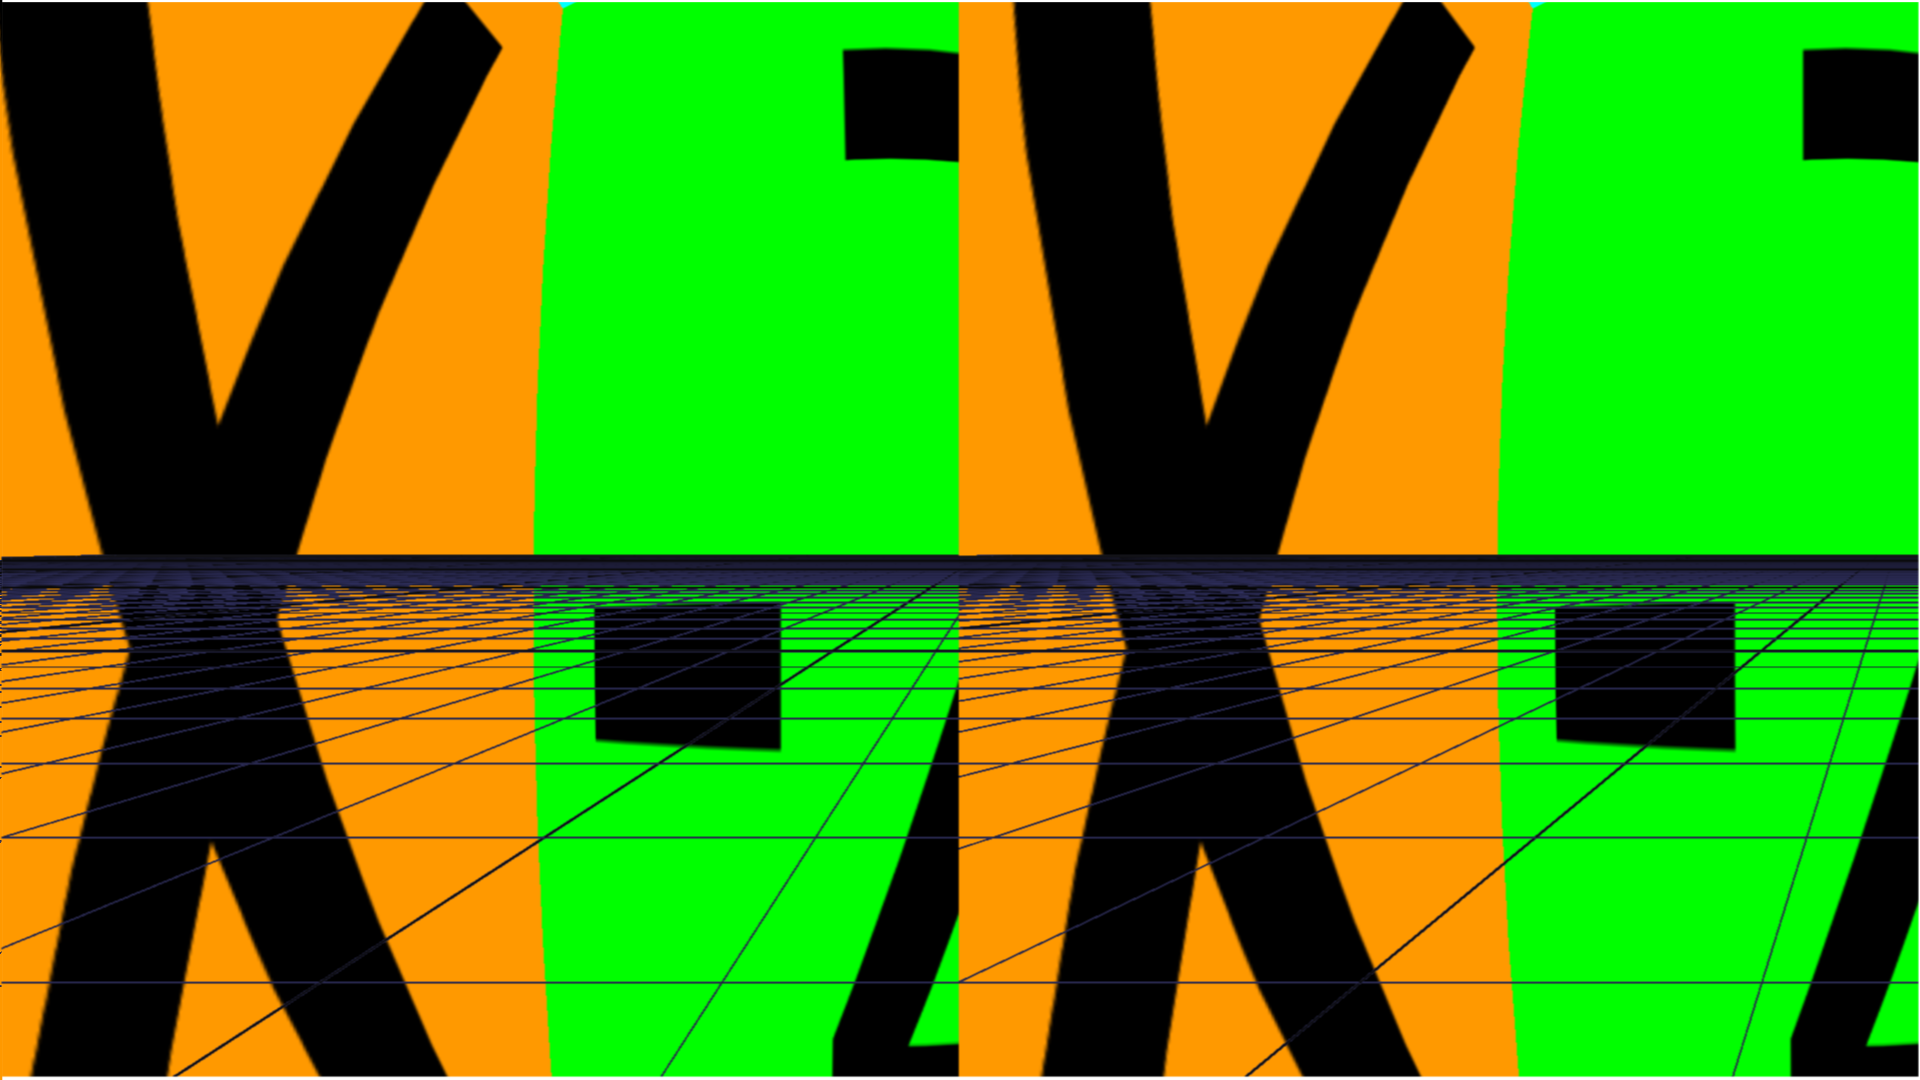
\includegraphics[width=0.45\linewidth,keepaspectratio=true]{figs/left_screen.png}&
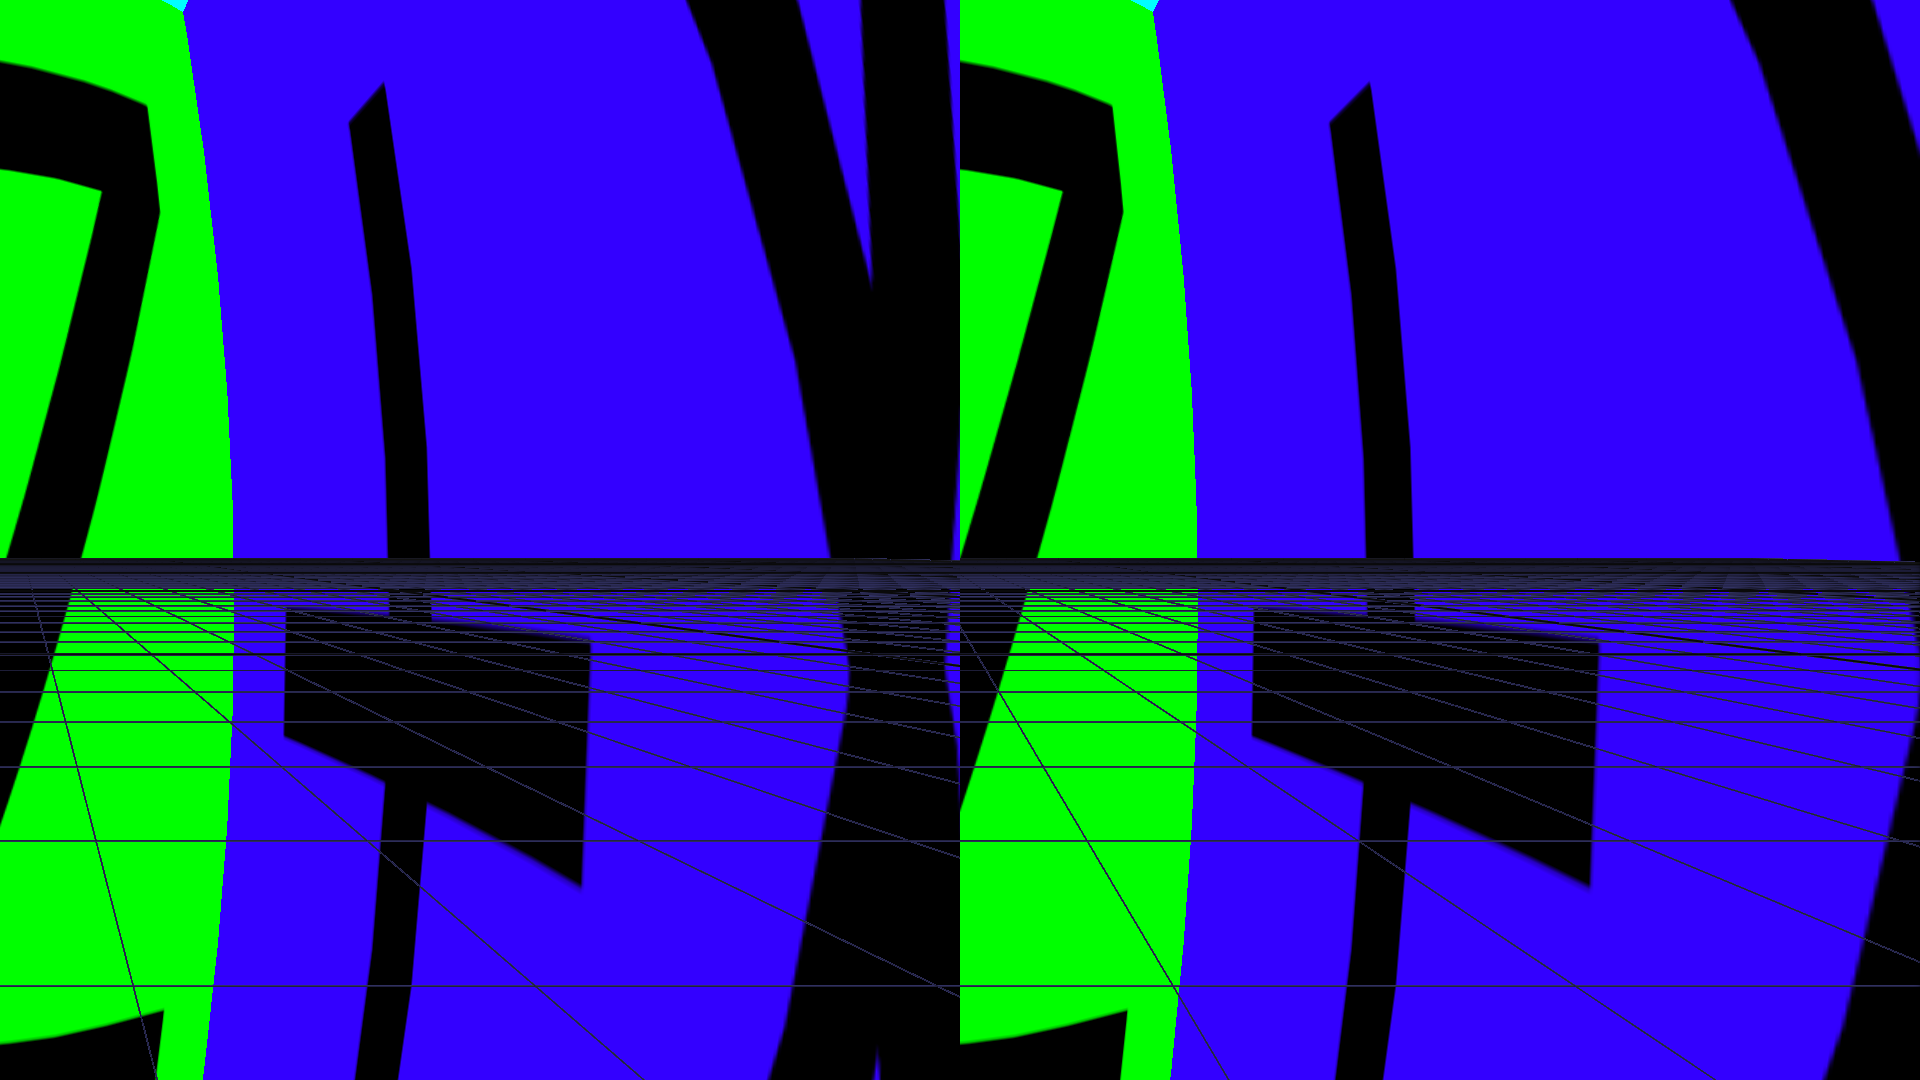
\includegraphics[width=0.45\linewidth,keepaspectratio=true]{figs/right_screen.png}\\
(a) Left display & 
(b) Right display
\end{tabular}
\caption{Vertical split of the stereo views.}
\label{fig.split_screens}
\end{figure}

The complete pipeline is described by Figure~\ref{fig.osg_pipeline}, where each box is a transformation. The bigger boxes are the view and projection transforms, $M_{cam}$ and  $M_{hcp}$, common for both screens. The smaller boxes are the transformations that specific for each screen and have different parameters, $M_{eye}$ and $M_{tilt}^{T}$ after $M_{cam}$; $M_{stereo}$ and $M_{off}$ after $M_{hcp}$.

\begin{figure}[!htb]
\centering
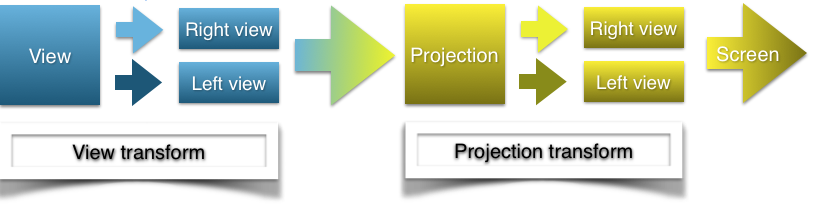
\includegraphics[width=0.9\linewidth,keepaspectratio=true]{figs/osg_pipeline.png}
\caption{The viewing pipeline for right and left views.}
\label{fig.osg_pipeline}
\end{figure}

%\section{Holographic Projection}
\label{sec.hologram_projection}

In the proposed holographic projection, the perspective projection is computed in a similar way, a 3D point in a truncated pyramid frustum (eye coordinates) is mapped to NDC; and the range of $x$ and $y$-coordinates from respectively $[l, r]$ and $[b, t]$ are still mapped to $[-1, 1]$, but the $z$-coordinate is mapped in the inverse way, from $[n, f]$ to $[1, -1]$. 

Note that the eye coordinates are still defined in the right-handed coordinate system, but now the camera at the origin is looking along $+Z$ axis in eye space, and along $+Z$ axis in NDC. The inversion of the $Z$  axis in Figure~\ref{fig.new_projection01} can be achieve by negating the third column of the projection matrix in Equation~\ref{eq.projection_matrix}.

%Since glFrustum() accepts only positive values of near and far distances, we need to negate them during the construction of \verb|GL_PROJECTION| matrix.

\begin{figure}[h!]
\centering
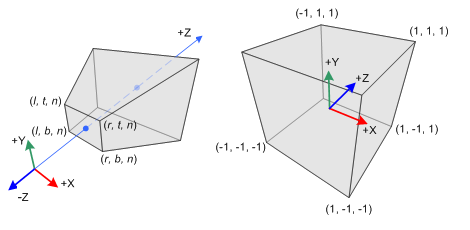
\includegraphics[width=0.9\linewidth,keepaspectratio=true]{figs/new_gl_projectionmatrix01.png}
\caption{Perspective Frustum and Normalized Device Coordinates (NDC)}
\label{fig.new_projection01}
\end{figure}


%The following diagrams show how a point $(x_e, y_e, z_e)$ in eye space is projected to $(x_p, y_p, z_p)$ on the near plane.

%\begin{figure}[!ht]
%\centering
%\begin{tabular}{cc}
%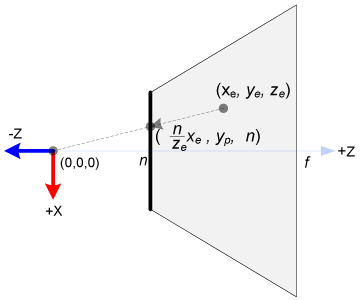
\includegraphics[width=0.45\linewidth,keepaspectratio=true]{figs/new_gl_projectionmatrix03.png}&
%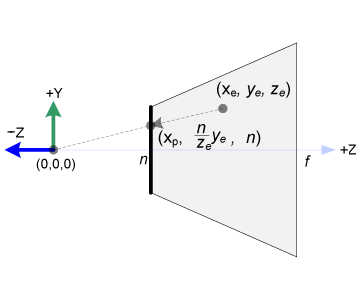
\includegraphics[width=0.45\linewidth,keepaspectratio=true]{figs/new_gl_projectionmatrix04.png}\\
%Top View of Frustum&
%Side View of Frustum
%\end{tabular}
%\caption{Views of the frustum.}
%\label{fig.new_frustum}
%\end{figure}

The permuted projection matrix is; 
\begin{equation}
\begin{aligned}
M^{\prime}_{proj} &= 
\begin{pmatrix} 
\frac{2n}{r-l} & 0 & -\frac{r+l}{r-l} & 0 \\
0 & \frac{2n}{t-b} & -\frac{t+b}{t-b} & 0 \\
0 & 0 & \frac{(f+n)}{f-n} & \frac{2fn}{f-n} \\
0 & 0 & 1 & 0 \\
\end{pmatrix} \\
\end{aligned}
\end{equation}



\section{Experiments and results}
\label{sec.results}

In this work the experiments used the OpenGL indirectly using the OpenSceneGraph~\cite{Burns2004}, a higher level, open-source, visualization framework. OpenSceneGraph provides a layer of abstraction over OpenGL in order to create the scene with memory managed objects, organized in a graph. This provides the dependencies of each object and optimises the memory utilization and rendering speed. Although the high-level of abstraction, it provides mechanisms to create custom operations if needed. The main advantage of using OpenSceneGraph for fishtank visualization is the easy abstraction with the windowing system, which is abstracted using object modeling strategy, and the multiple displays infrastructure. The visualization pipeline for the left and right screens introduces independent transformations for each screen defined by slave cameras. Each slave camera has view and projection transformations for each screen. In usual cases, those slave cameras are used to create a powerwall composed by many screens. The Figure~\ref{fig.osg_pipeline} show a schematic illustration of the pipeline for dual screens which are used to emulate an hologram, where the small arrows represent the slave cameras.

\begin{figure}[!hb]
\centering
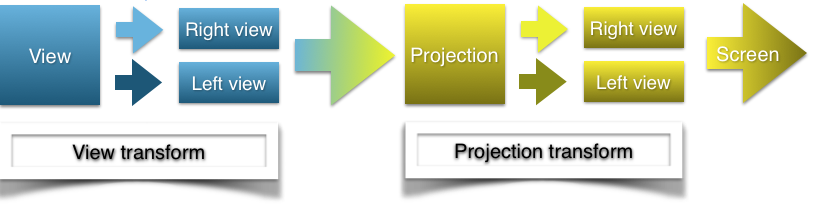
\includegraphics[width=\linewidth,keepaspectratio=true]{figs\osg_pipeline.png}
\caption{The viewing pipeline of OpenSceneGraph.}
\label{fig.osg_pipeline}
\end{figure}

In this investigation, a setup of two 3D displays forming a fish tank as in the illustration of Figure~\ref{fig.tv_setup}a. The fish tank has an extended field of view (FOV) of $120$ degrees between the displays, as illustrated in Figure~\ref{fig.tv_setup}b. They show the scene accordingly the view point of the viewer. The  position of the face of the viewer is tracked using a depth camera, in this case the Microsoft Kinect Sensor, and the viewer can use any of the stereo technologies presented in Section~ref{sec.stereo}. One drawback is the limitation of only one user but it can be overcome with a new display technology developed by Microsoft Research~\cite{Harris2010}. In order to create the space where the hologram is shown, the unconnected sides of the displays form the sides of a virtual 3D display where the origin of the hologram projected. The Figure~\ref{fig.tv_setup} show the setup of the experiment, with 2 stereo displays and the Kinect sensor. The area of tracking is shown by the frustum coming from the sensor. The original setup had 2 kinect sensors placed on the base of each display, but due hardware constrains, the setup has been reduced to only on sensor. The effect of this is a smaller tracking area, but it can be easily extended with extra hardware.

\begin{figure}[!ht]
\centering
\begin{tabular}{cc}
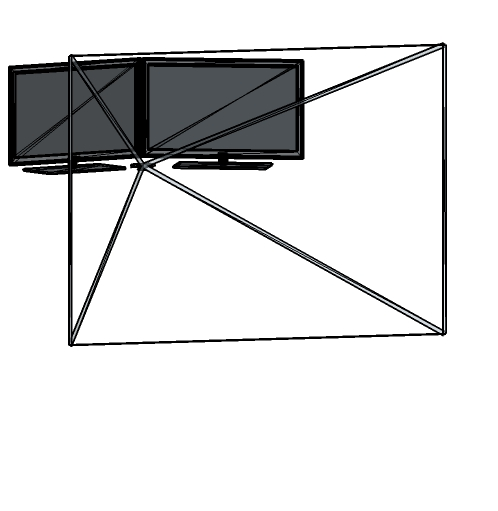
\includegraphics[width=0.45\linewidth,keepaspectratio=true]{figs\tv_setup_01.jpg}&
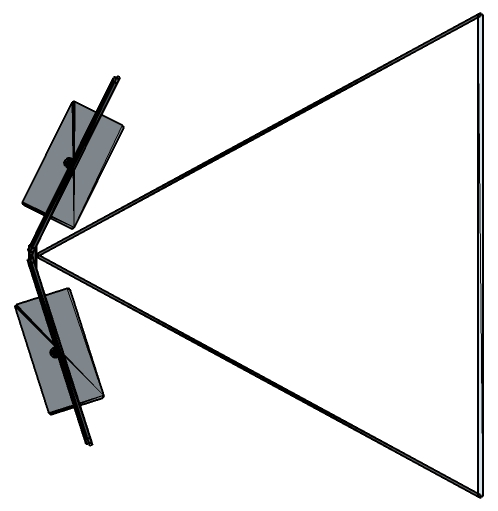
\includegraphics[width=0.45\linewidth,keepaspectratio=true]{figs\tv_setup_02.jpg}\\
(a) Stereo displays and Kinect & 
(b) Top view of fishtank
\end{tabular}
\label{fig.tv_setup}
\caption{Setup of the stereo displays and Kinect sensor}
\end{figure}

The implementation of the experiment used a face tracking library available in the Kinect SDK from Microsoft~\cite{Zhang2012}, which can track faces without prior training. The software can adjust the pitch angle of the sensor while it keeps the face in the center of the image. Ir order to remove the noise, the tracked movement is filtered by a step function in Equation{eq.step} ; that takes displacements $x$ greater than 1 cm or the average of the displacements $\mu_x$ if smaller. The Figure~\ref{fig.tracking} shows, on the right side, the video used in the face tracking and an overlay of a mask projected on of the video with the distance tracked. The attitude of the viewer, shown in the avatar on the left, is not used in this work because the hologram should stay on the same position for any rotation of the face.

\begin{equation}
  u(x)=\begin{cases}
    x, & \text{if $x>1$}.\\
    \mu_{x}, & \text{otherwise}.
  \end{cases}
  \label{eq.step}
\end{equation}

\begin{figure}[!ht]
\centering
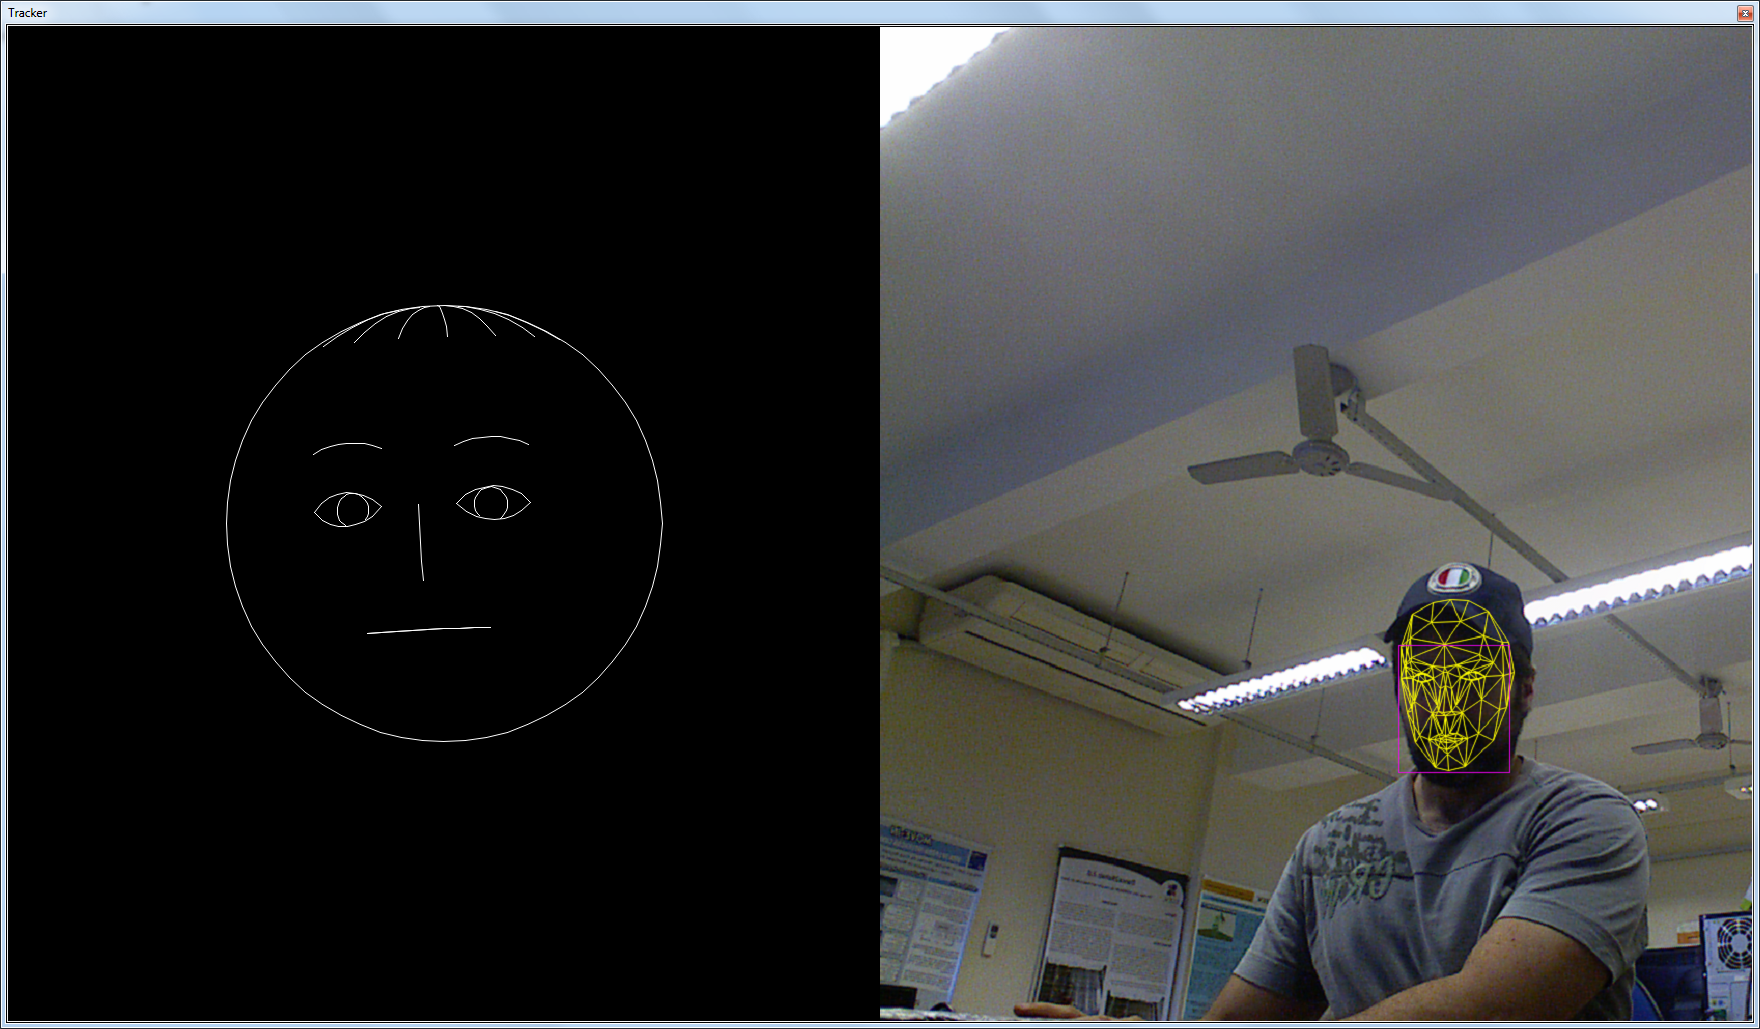
\includegraphics[width=0.9\linewidth,keepaspectratio=true]{figs\tracking.png}
\label{fig.tracking}
\caption{Face tracking module used to track the position of the viewer.}
\end{figure}

The stereo rendering uses the horizontal half of each screen for each eye as shown in Figure~\ref{fig.screens}. The projection is displaced by a horizontal offset on each slave view (small arrows) in projection transform of Figure~\ref{fig.osg_pipeline}. The width of bezel of the displays is taken in account in the offset to preserve an hidden continuity between the displays. The rotation of the screens is placed in slave cameras in the view transform.

\begin{figure}[!ht]
\centering
\begin{tabular}{cc}
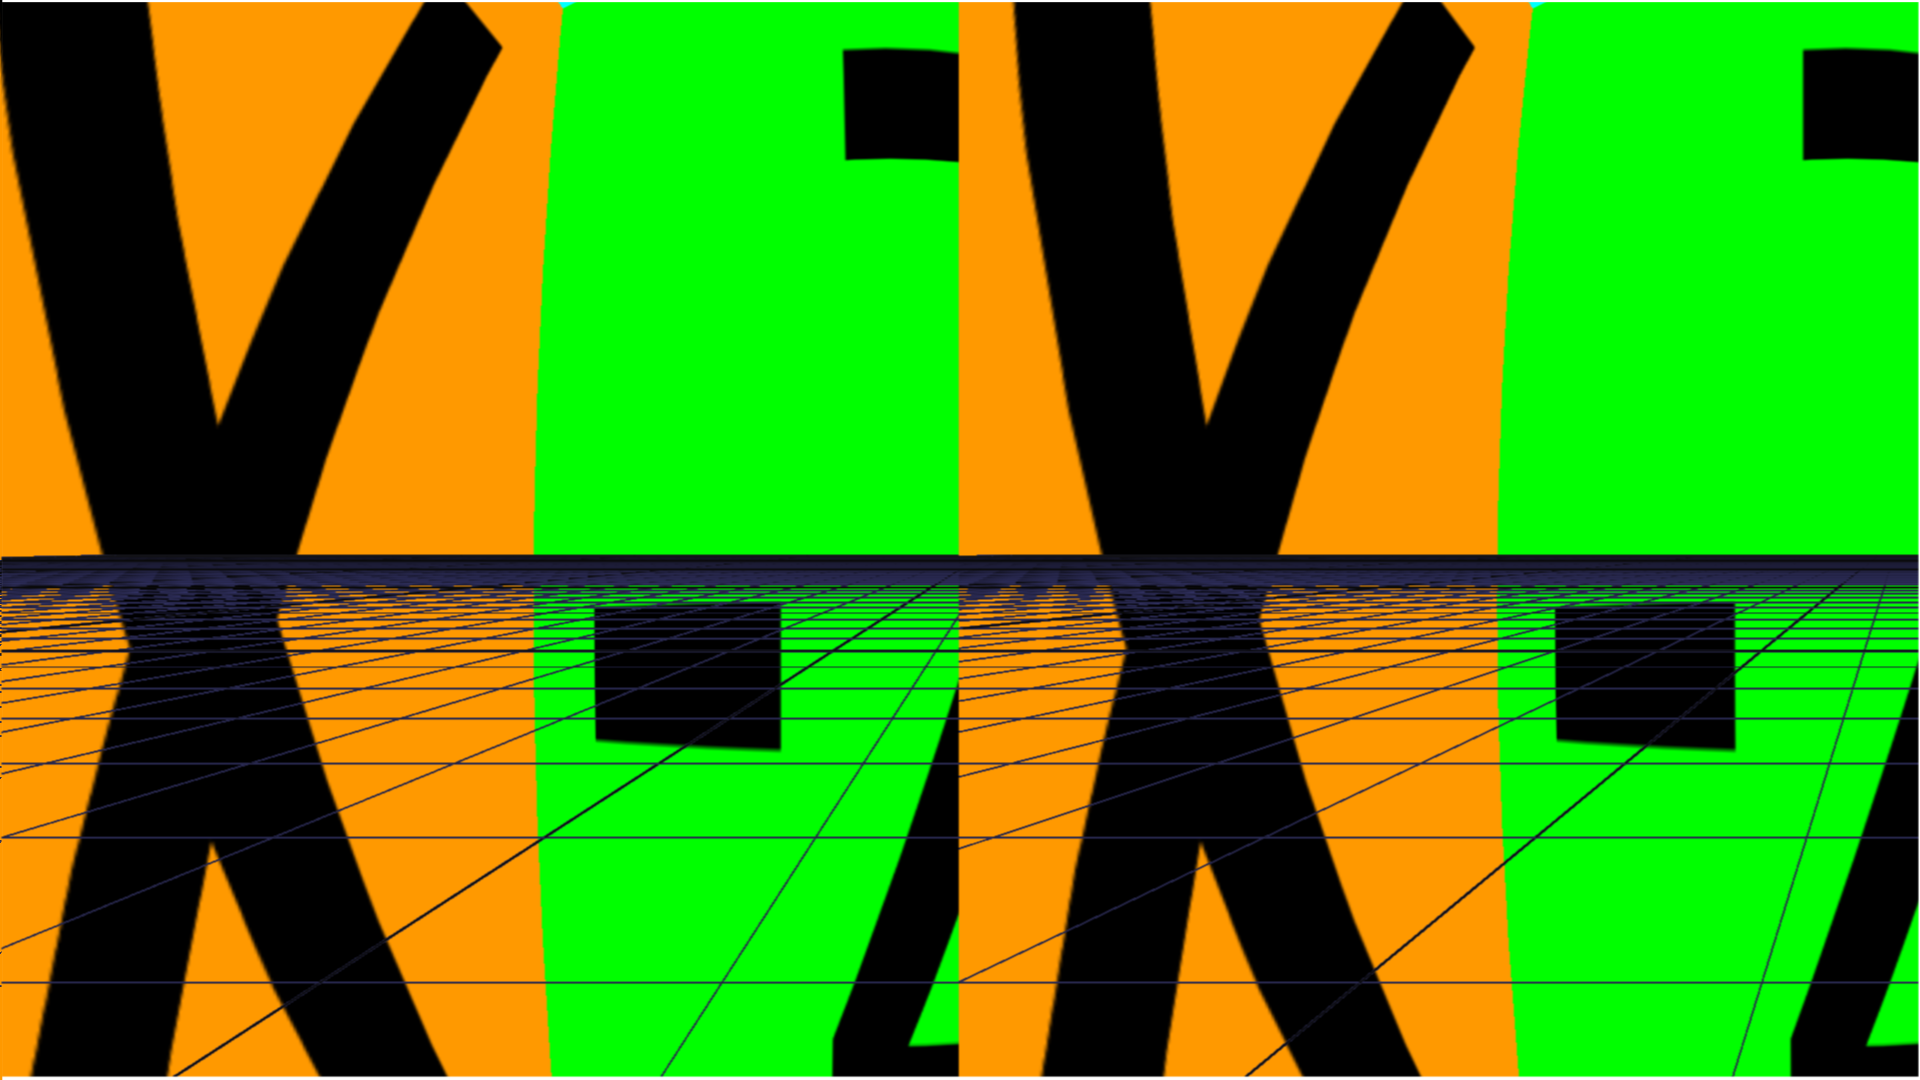
\includegraphics[width=0.45\linewidth,keepaspectratio=true]{figs\left_screen.png}&
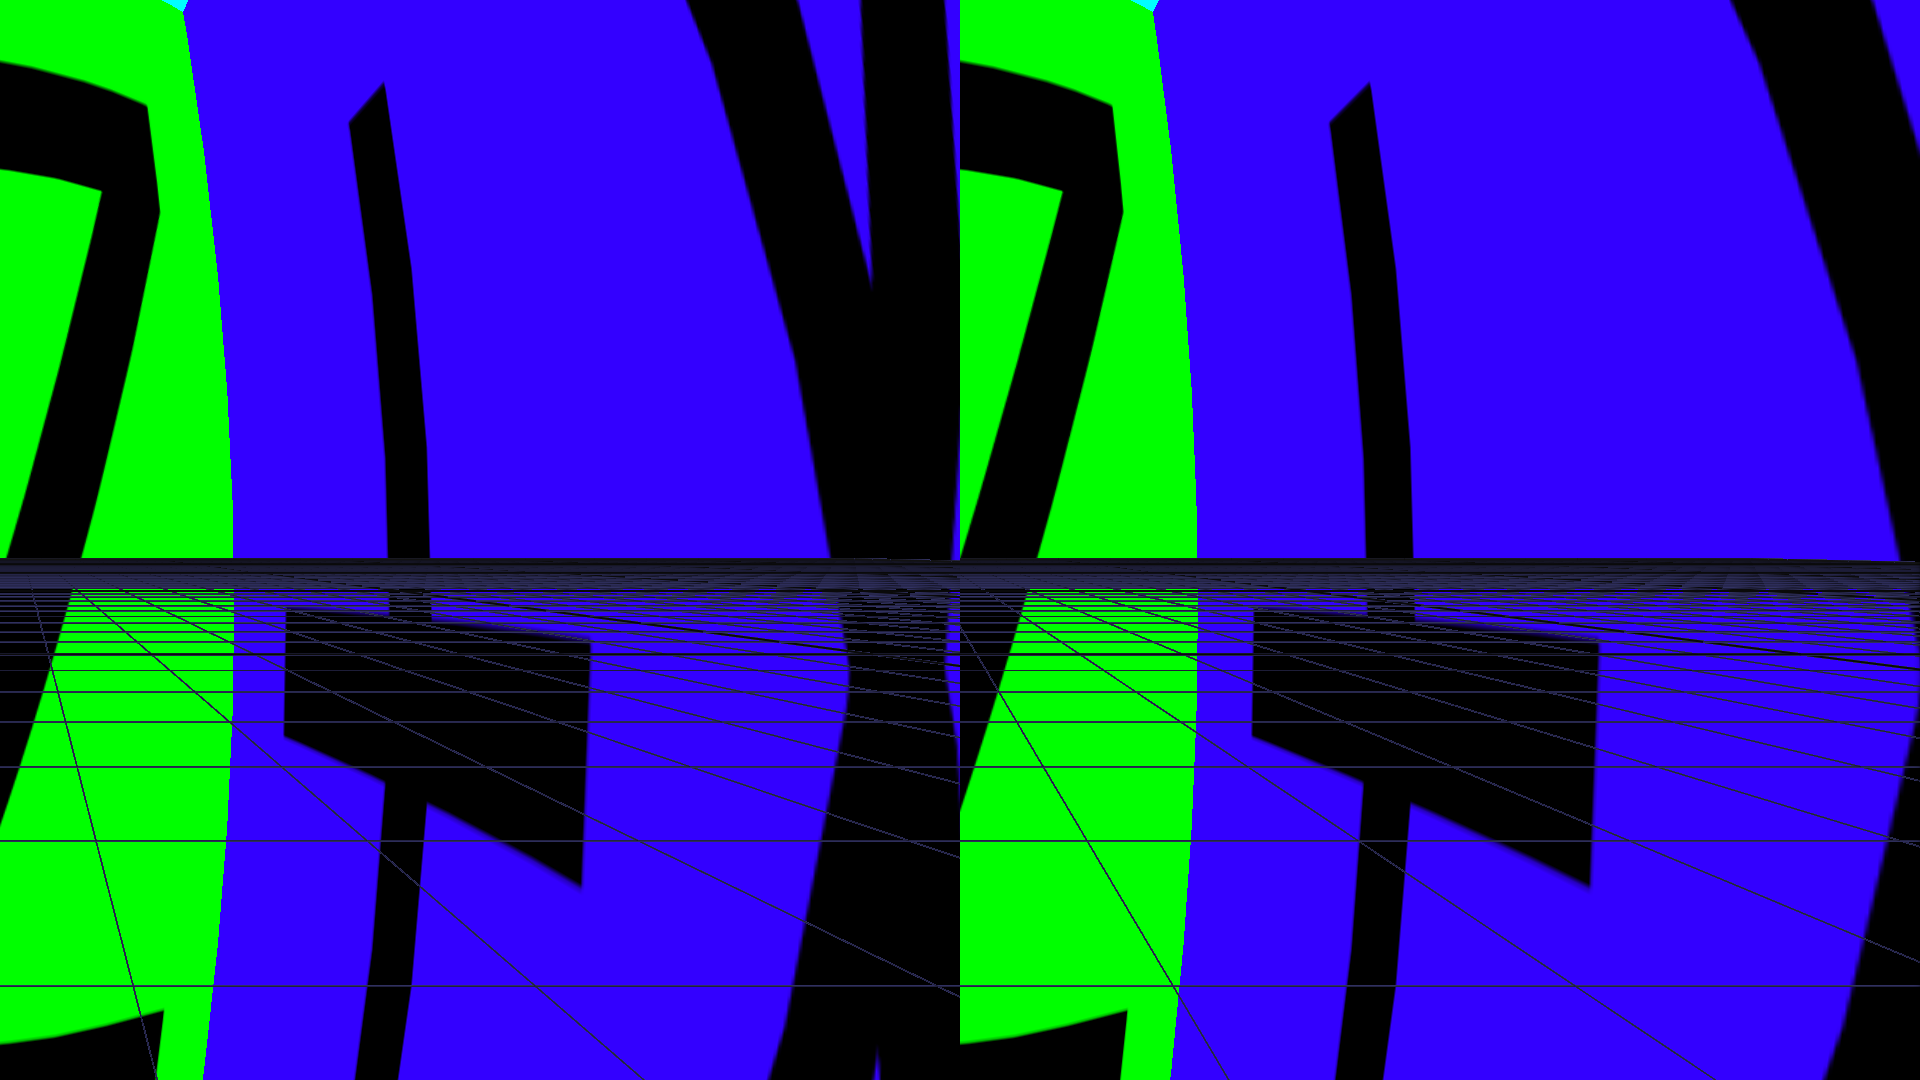
\includegraphics[width=0.45\linewidth,keepaspectratio=true]{figs\right_screen.png}\\
(a) Left display & 
(b) Right display
\end{tabular}
\label{fig.screens}
\caption{Vertical split of the stereo views.}
\end{figure}

The results of the experiments successfully emulated an hologram using the procedure described in Section~\ref{sec.hologram_emulation}, which changes the attitude of the models on the scene to produce the correct viewpoint. The experiments with the holographic projection transform are left for future work.







\section{Conclusion}
\label{sec.conclusion}

This work presented the principles behind the generation of an holographic and stereo visualization. The first is still not consolidated because it needs special hardware and high computational power; but it has the benefit of reproducing the light in all directions, from all viewpoints. The latter is a visualization technique already present in the stereo monitors, TVs and movie screens; but with a limited immersion due the the fixed viewpoint.

The new projection transformation for stereo displays using the OpenGL framework creates the illusion of an hologram. The human stereo vision requires only two viewpoints of the hologram, it was emulated in the stereo displays. The viewpoint is adjusted in real-time with the tracked position of the viewer.

The experiment shows a computer generated projection in a fishtank setup composed by two stereo displays. The hologram is emulated using negative stereo parallax and high precision tracking of the viewer. The holographic emulation is an effort to use the current technology to produce the same immersion of visualization of an hologram. New development in holographic technology will allow holographic displays, but will take at least half decade in order to have commercial products with this technology. The cost of the high end hardware necessary to create CGH are not yet proportional to the needs of this visualization technique, and this work shows that holographic immersive environment can be done today with out-of-the-shelf hardware. The  stereo displays and Kinect sensor are available for a fraction of the cost of a special hardware.



\bibliographystyle{IEEEtranN}
\bibliography{references}
\end{document}